% Preamble and some settings
\documentclass[letterpaper]{article}

% Geometry
\usepackage[letterpaper, top=2.54cm, bottom=2.54cm, left=2.54cm, right=2.54cm]{geometry}

% Fancy Header
\usepackage{fancyhdr}
% Change header bottom bar thickness
\renewcommand{\headrulewidth}{0pt}

% Hyperlinks
% -option hidelinks disables red boxes around links
\usepackage[hidelinks]{hyperref}

% Colours
\usepackage{color}
% define before tikz or pstricks
\usepackage[usenames,dvipsnames]{xcolor}
\definecolor{grey}{gray}{0.4}

% For pictures
\usepackage{graphicx}

% For special character support
\usepackage[utf8]{inputenc}
\usepackage[T1]{fontenc}

% New center environment with no padding
\newenvironment{centernop}[1][\topsep]
  {\setlength{\topsep}{#1}\par\kern\topsep\centering}% \begin{centernop}[<len>]
  {\par\kern\topsep}% \end{centernop}

% New bottom paragraph environment
\newenvironment{bottompar}{\par\vspace*{\fill}}{\clearpage}

% Tikz
\usepackage{tikz}
\usetikzlibrary{positioning}


% Landscape pages
\usepackage{lscape}

% Phylogenetic Trees
% -http://cbr.jic.ac.uk/dicks/software/newicktree/
% -requires compiling with xelatex
%\usepackage{newicktree}

% Qtree
%\usepackage{qtree}

% Enumitem for formatting enumerated lists
\usepackage{enumitem}

% For hanging indents
\usepackage[notquote]{hanging}

% Listings
\usepackage{listings}
\lstset{
	tabsize=2,
	basicstyle=\ttfamily,
	aboveskip=0pt,
	belowskip=\baselineskip
}

% requires --shell-escape
\usepackage{minted}

% Courier
% -for \ttfamily to work in listings
\usepackage{courier}

% Paragraph box
\usepackage{pbox}

% Math symbols and other symbols
\usepackage{amsfonts}
\usepackage{amssymb}

% Math tools
\usepackage{mathtools}
% \ceil{} and \floor{} functions
\DeclarePairedDelimiter\ceil{\lceil}{\rceil}
\DeclarePairedDelimiter\floor{\lfloor}{\rfloor}

% Tilde macro
\newcommand{\mytilde}{\raise.17ex\hbox{$\scriptstyle\mathtt{\sim}$}}

% Margin paragraph commands
\DeclareRobustCommand{\mymarginpar}[1]{%
 \mbox{}\marginpar[\raggedleft#1]{\raggedright#1}
 \vspace{-\baselineskip}
}
\DeclareRobustCommand{\mpconsider}{%
 \mymarginpar{\textit{Consider}}
}
\DeclareRobustCommand{\mpclaim}{%
 \mymarginpar{\textbf{Claim}}
}
\DeclareRobustCommand{\mpex}{%
 \mymarginpar{Ex.}
}
\DeclareRobustCommand{\mpnote}{%
 \mymarginpar{\textit{Note}}
}
\DeclareRobustCommand{\mpproof}{%
 \mymarginpar{\textbf{Proof}}
}
\def\mpreadings{\mymarginpar{\textit{Readings}}}
\def\mpselftest{\mymarginpar{\textit{Self test}}}

% Quick Commands
\def\N{\mathbb{N}}
\def\R{\mathbb{R}}
\def\implies{\Rightarrow}
\def\and{\wedge}
\def\Or{\vee}

\graphicspath{{./figures/}}

\hypersetup{
    colorlinks=true,
    linkcolor=black,
    urlcolor=cyan
}

% Title
\title{MetaFlux: A Dank Framework}
\author{iGEM UofT}
\date{Julian Mazzitelli}

% Remove title from table of contents
\renewcommand*\contentsname{}

% Link shortcuts
\def\Blender{\href{https://www.blender.org/}{Blender}}

% Italicization shortcuts
\def\MetaFlux{\textit{MetaFlux}}
\def\SMBL{\href{http://sbml.org/Main_Page}{SMBL}}

\begin{document}

\maketitle

% \thispagestyle{empty}

% \begin{bottompar}
% \tableofcontents
% \end{bottompar}

% \newpage
% \setcounter{page}{1}

\section{Introduction}

Given the rapid advancements in genome-scale reconstructions and metagenomics
over the past several years [ref.], there is a need to effectively and succintly
analyze and interpret this data. We present \MetaFlux, a web based tool for
visualing, modifying, and comparing analyses of genome scale metabolic models.
\MetaFlux\ can dynamically present community level interactions as well as single
species models. [How to write as one sentence?]

\section{Data}

\MetaFlux\ visualizes genome models. Currently, the models available within our
app are \textit{Systems Biology Markup Language} (\SMBL) formatted models as
\texttt{xml} files taken from the literature [refs.]. We are interested in
incorporating autogenerated models from tools such as MicrobesFlux and Model
SEED in the future. Morever, the ability for a user to upload a model will be
implemented.

\subsection{Model Schema For Single Species}

The following is a BSON implementation of an SMBL metabolite model schema which
can be saved in a MongoDB NoSQL database. The following snippet is directly
operable within a NodeJS environment.

\inputminted{js}{snippets/MetabolicModel.js}

These are all of the properties present in the literature retreived models.
However, further attributes (such as \texttt{flux\_value}) will be appended
into the model.

\subsection{Model Schema for Community Structure}

In our community level representations, different species are described using
seperate compartments. Reactions involving shared extracellular metabolites
are constructed for each specie to mediate meteabolite exchange through the
extracellular space.

\section{Visualization}

From a community level, one may see the following visualization:

\begin{center}
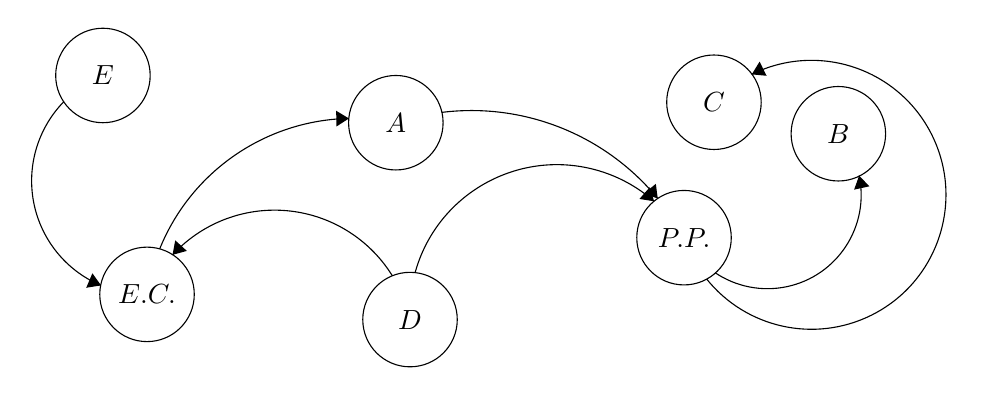
\begin{tikzpicture}[scale=0.2]
\tikzstyle{every node}+=[inner sep=0pt]
\draw [black] (15.6,-29.4) circle (3);
\draw (15.6,-29.4) node {$E.C.$};
\draw [black] (49.7,-25.8) circle (3);
\draw (49.7,-25.8) node {$P.P.$};
\draw [black] (31.4,-18.5) circle (3);
\draw (31.4,-18.5) node {$A$};
\draw [black] (59.5,-19.2) circle (3);
\draw (59.5,-19.2) node {$B$};
\draw [black] (51.6,-17.2) circle (3);
\draw (51.6,-17.2) node {$C$};
\draw [black] (32.3,-31) circle (3);
\draw (32.3,-31) node {$D$};
\draw [black] (12.8,-15.5) circle (3);
\draw (12.8,-15.5) node {$E$};
\draw [black] (16.403,-26.516) arc (157.97288:91.22865:13.27);
\fill [black] (28.42,-18.23) -- (27.61,-17.74) -- (27.63,-18.74);
\draw [black] (34.322,-17.843) arc (97.06113:39.44405:15.316);
\fill [black] (48.03,-23.31) -- (47.91,-22.38) -- (47.14,-23.01);
\draw [black] (60.819,-21.859) arc (11.93817:-124.02005:5.95);
\fill [black] (60.82,-21.86) -- (60.5,-22.75) -- (61.47,-22.54);
\draw [black] (54.001,-15.428) arc (116.36436:-141.28085:8.539);
\fill [black] (54,-15.43) -- (54.94,-15.52) -- (54.5,-14.62);
\draw [black] (32.621,-28.03) arc (-195.36977:-311.35262:9.343);
\fill [black] (47.8,-23.49) -- (47.53,-22.59) -- (46.87,-23.34);
\draw [black] (17.22,-26.892) arc (137.37213:31.68245:8.801);
\fill [black] (17.22,-26.89) -- (18.13,-26.64) -- (17.39,-25.97);
\draw [black] (12.676,-28.833) arc (-112.89802:-224.32362:7.209);
\fill [black] (12.68,-28.83) -- (12.13,-28.06) -- (11.74,-28.98);
\end{tikzpicture}
\end{center}


In the above graphic each arrow represents an enzmyatic mediated reaction.
\textit{E.C.} represents the species \textit{E. Coli} and \textit{P.P.}
represents \textit{P. Putida}. \textit{A} is a metabolite exported by
\textit{E.C} and imported by \textit{P.P}. \textit{B} and \textit{C} are
metabolites exported by \textit{P.P.} \textit{D} is a metabolite which is
imported by both species, and potentially conferring to a competitive
relationship. Finally, \textit{E} is a metabolite imported into \textit{E.
Coli}. We arrive at set of potential relationships between two species
\textit{a,b} and a metabolite \textit{m}:

\begin{itemize}

\item Single species exporting a metabolite: $\{a,b\} \rightarrow m$
\item Single species importing a metabilte: $m \rightarrow \{a,b\}$
\item Synergistic export/import between two species: $\{a \rightarrow m \rightarrow b, b \rightarrow m \rightarrow a \}$
\item Competition for a metabolite between two species: $\{m \rightarrow a,b \}$

\end{itemize}

Given the above definition, we can generalize to any number of ``compartments''
and any number of metabolites. Furthermore, this additionally provides the means
to segregate the intracellular compartments of a single species model, such as
the cytosol, periplasm, and internal subsystems. The ability to create new
subsystems from within the web interface will be added in a later release.

\section{Graph Construction}

Once we have been provided with model data in the schema format as described
above, so begins the graph construction process. This process aims to be
as parametizable and generalizable as possible, in order to accomodate
the creation of custom groupings.

The first thing to do is construct \texttt{Metabolite} and \texttt{Reaction}
objects.

\begin{minted}{coffee}
buildPeices = (model) ->
    nodes = {}, reactions = {}

    for metabolite in model.metabolites
        nodes[metabolite.id] = new Metabolite(metabolite, ...)

    for reaction in model.reactions
        reactions[reaction.id] = new Reaction(metabolite, ...)

        for metabolite of reaction.metabolites
            if reaction.metabolites[metabolite] > 0
                source = reaction.id
                target = metabolite
            else
                source = metabolite
                target = reaction.id

            reactions.addLink(new Link(source, target, ..))
\end{minted}

After this is done, we have two dictonaries storing all metabolites and
reactions that will be used to construct our system. The next step is to use the
prototype methods of the \texttt{Reaction} object to construct ``compartments''
as necessary. This will be done recursively, and with paramaters and defaults
outling the sets of compartments. For example, one set could be $\{E.C.,
extracellular, P.P.\}$, while another, nested within \textit{E.C.} could be
$\{cytosol, periplasm, extracellular\}$.

\begin{minted}{coffee}

# Will be called recursively
# The first call will pass in nodes, reactions
# set of reaction types? can be built w/ reactions
# Constructs a graph object
compartmentatilization = (system) ->
    # TODO

\end{minted}

\end{document}
